	\begin{Huge}
			Informatik
		\end{Huge}
		\begin{exampleblock}{\textcolor{white}{Was ist der Studiengang?}}
			Der grundständigste *-Informatik-Studiengang. Beinhaltet im Gegensatz zu anderen Studiengängen den meisten Umgfang an technischer und theoretischer Informatik. Eine gute Portion Mathe ist außerdem dabei. Außerdem beinhaltet die Informatik ein beliebig wählbares Schwerpunktfach (das nicht Sport sein darf).
		\end{exampleblock}
	
	\begin{block}{Welcher Teil macht wie viel im Studium aus?}
		\begin{figure}[h!]
			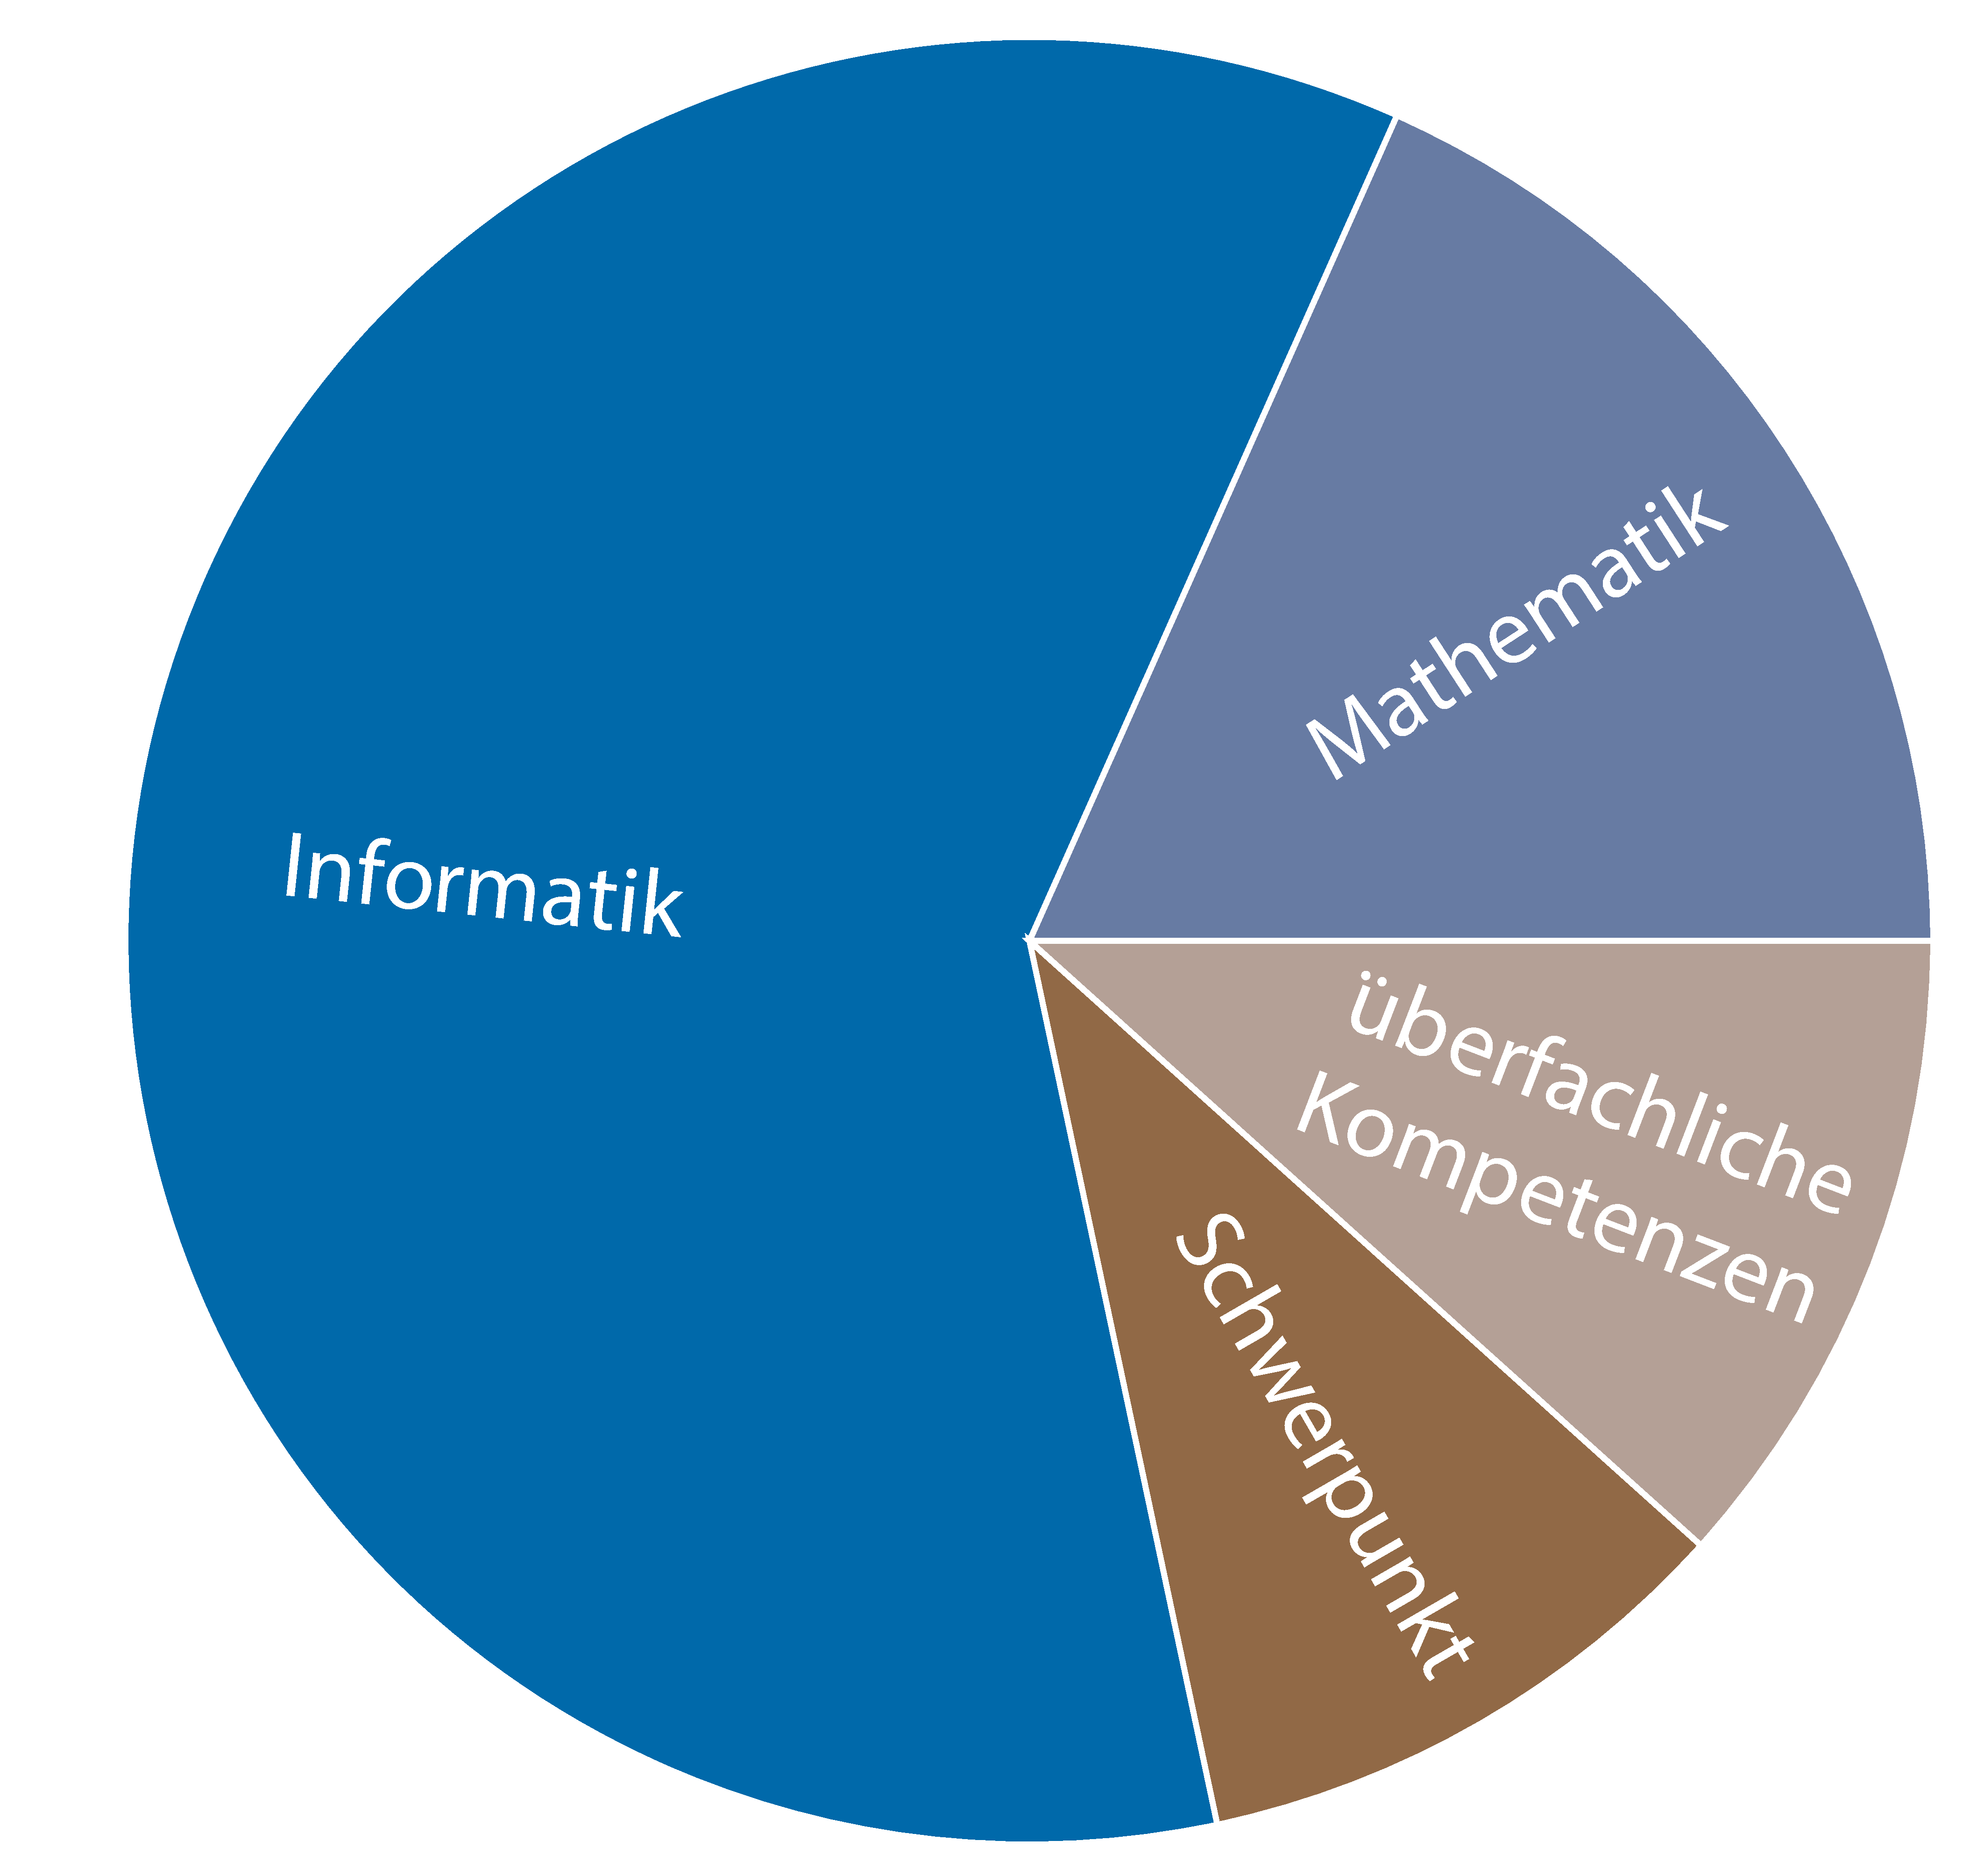
\includegraphics[width=0.4\textwidth]{charts/informatik-Piechart.pdf}
			\caption{Verteilung der Themenbereiche über das komplette Studium}
		\end{figure}
	\end{block}
	
	\begin{block}{Was macht man in welchem Semester?}
		\begin{figure}[h!]
			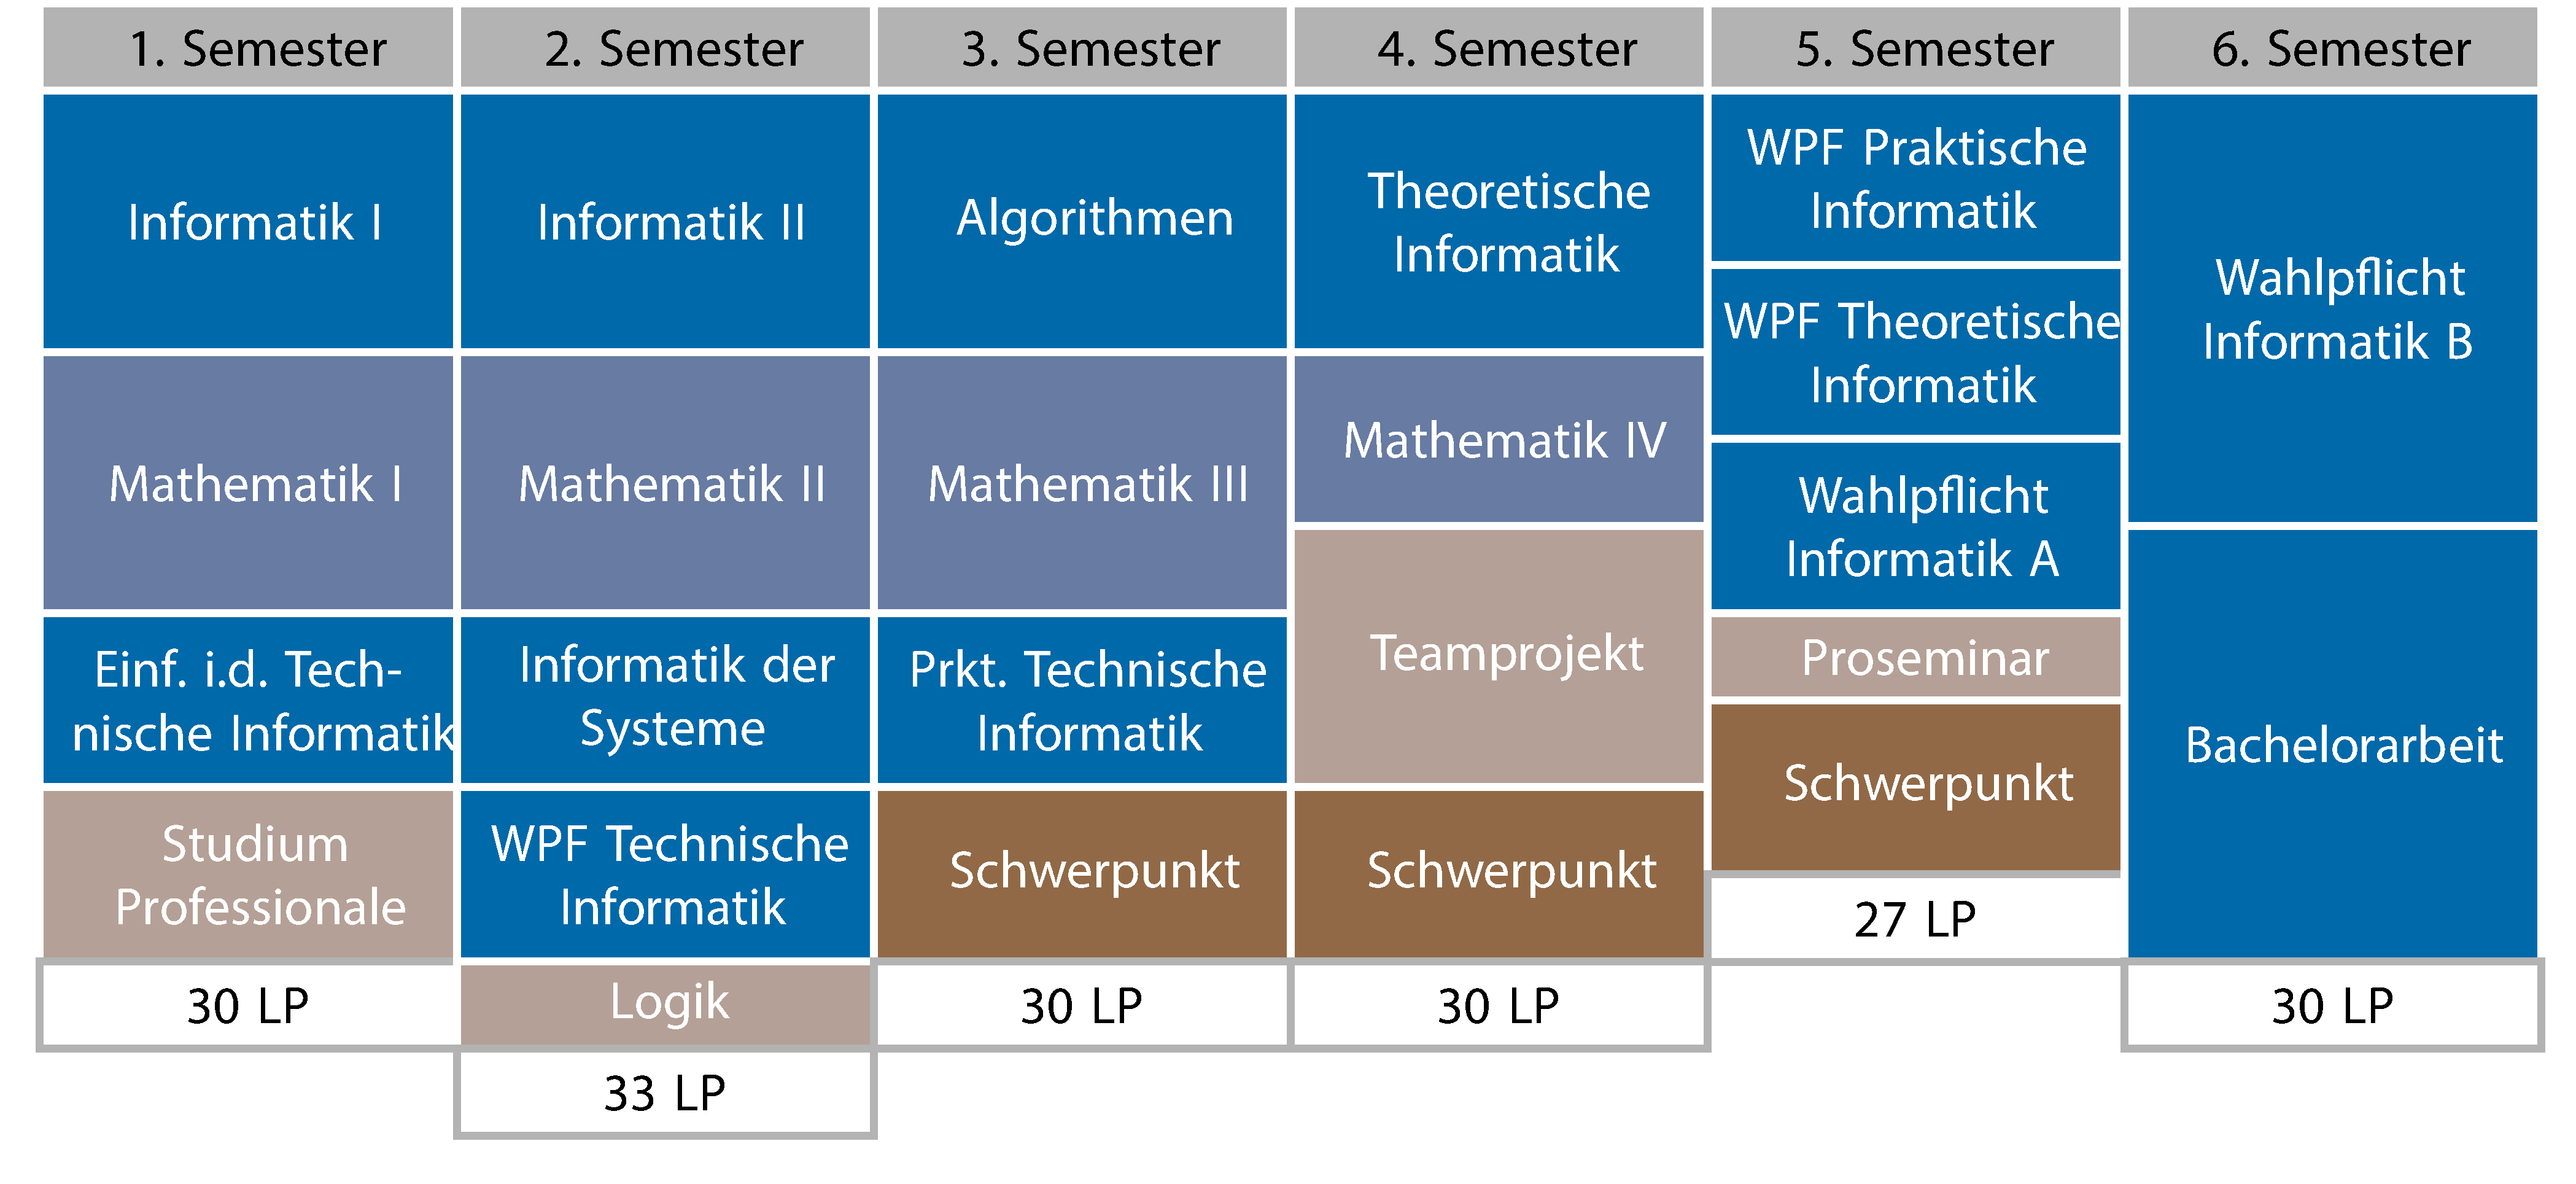
\includegraphics[width=\textwidth]{charts/informatik-Studienplan_abWS18.pdf}
		\end{figure}
		Dieser Verlauf ist allerdings nur ein Vorschlag und kein bindender Studienplan. Es empfiehlt sich jedoch, den Plan einzuhalten, wenn man in Regelstudienzeit studieren möchte.
	\end{block}
